The cart subsystem is largely the cart itself. it shall have pace for carrying user tools together with a charging area for user to put charging equipment, kill switch, manual mode switch and the wheels.

\subsection{MANUAL MODE SWITCH SUBSYSTEM}
The manual mode switch subsystem will be used to switch the cart to manual mode by disconnecting the power supply to the crab drive
\begin{figure}[h!]
	\centering
 	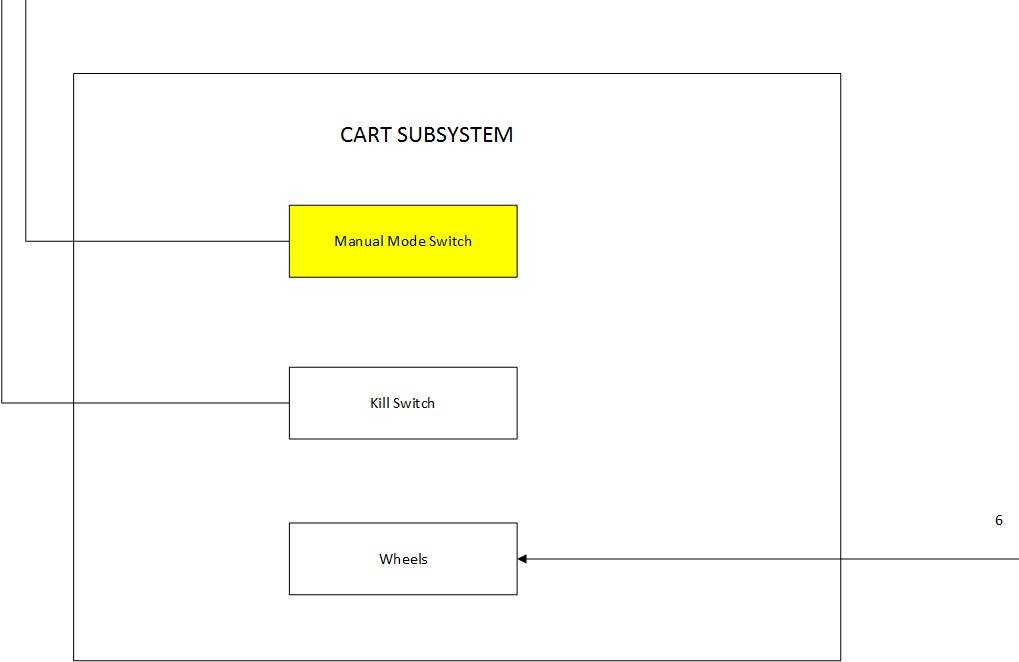
\includegraphics[width=0.60\textwidth]{images/manualmodeswitch}
 \caption{Manual Switch subsystem description diagram}
\end{figure}

\subsubsection{ASSUMPTIONS}
Assumptions made are as follows:
\begin{itemize}
\item The manual mode switch subsystem will ensure the safety of users and around the user
\item The manual mode switch subsystem will not power off Smart Cart, but simply disable autonomous motion  
\end{itemize} 

\subsubsection{RESPONSIBILITY}
The manual mode switch subsystem responsibilities are as follows:
\begin{itemize}
\item The switch will be used to disable the autonomous motion of the cart.
\item The switch will ensure safety of the users and the surrounding people
\end{itemize}

\subsubsection{Manual Mode Subsystem Interface}
\begin{table}[H]
\caption{Manual mode switch subsystem interface}
\begin{center}
\begin{tabular}{ | p{1cm} | p{6cm} | p{3cm} | p{3cm} |}
    \hline
    ID & Description & Inputs & Outputs \\ \hline
    \ N/A & Disable converter & \pbox{3cm}{N/A} & \pbox{3cm}{Voltage converter}  \\ \hline
\end{tabular}
\end{center}
\end{table}


\subsection{KILLSWITCH}
The killswitch subsystem will be used to ensure that the Smart Cart will be immediately turned off.
\begin{figure}[h!]
	\centering
 	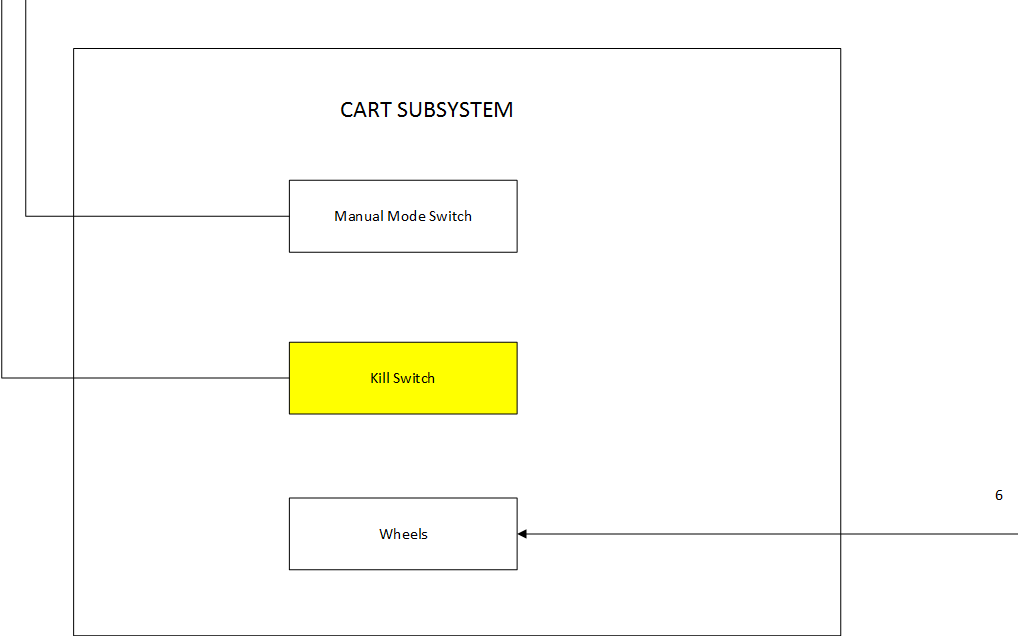
\includegraphics[width=0.60\textwidth]{images/killswitch}
 \caption{Kill Switch subsystem description diagram}
\end{figure}

\subsubsection{Assumptions}
Assumptions made are as follows:
\begin{itemize}
\item Power to Smart Cart components will be disabled
\item Power to external tools and equipment will be disabled
\end{itemize}

\subsubsection{RESPONSIBILITIES}
The killswitch subsystem responsibility are as follows:
\begin{itemize}
\item the switch will disable the battery from powering Smart Cart and its components
\end{itemize}

\subsubsection{Killswitch subsystem interface}
\begin{table}[H]
\caption{Sensors subsystem interface}
\begin{center}
\begin{tabular}{ | p{1cm} | p{6cm} | p{3cm} | p{3cm} |}
    \hline
    ID & Description & Inputs & Outputs \\ \hline
    \ N/A & Disable battery & \pbox{3cm}{N/A} & \pbox{3cm}{Deep cycle battery }  \\ \hline
\end{tabular}
\end{center}
\end{table}

\subsection{WHEEL SUBSYSTEM}
The wheels subsystem will be used to provide movement to the Smart Cart. The wheels will be controlled by the Crab Drive layer.
\begin{figure}[h!]
	\centering
 	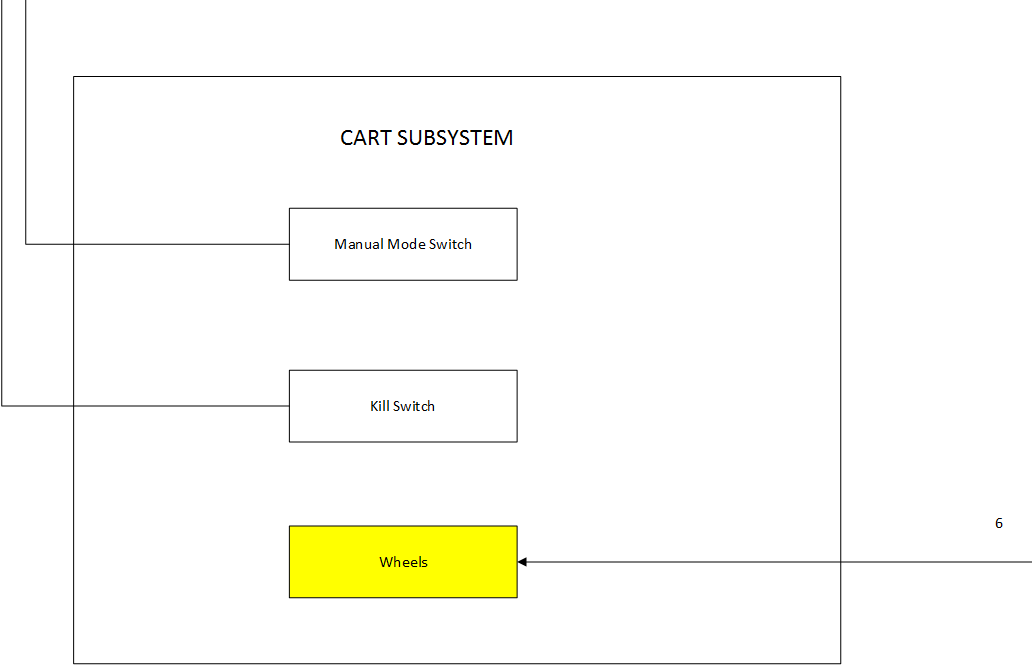
\includegraphics[width=0.60\textwidth]{images/wheels}
 \caption{Wheels subsystem description diagram}
\end{figure}

\subsubsection{ASSUMPTIONS}
Assumptions made are as follows:
\begin{itemize}
\item The wheels will be able to turn in the direction sort
\item The wheels will move harmoniously
\end{itemize}

\subsubsection{RESPONSIBILITIES}
The wheel subsystem responsibilities will be as follows
\begin{itemize}
\item Turn and move the cart from one point to anther
\item Take turns as directed by the wheel motors
\end{itemize}

\subsubsection{Wheel subsystem interfaces}
\begin{table}[H]
\caption{Sensors subsystem interface}
\begin{center}
\begin{tabular}{ | p{1cm} | p{6cm} | p{3cm} | p{3cm} |}
    \hline
    ID & Description & Inputs & Outputs \\ \hline
    \ 5 & Move Smart Cart & \pbox{3cm}{Wheel Motors} & \pbox{3cm}{N/A}  \\ \hline
\end{tabular}
\end{center}
\end{table}

